\setlength\intextsep{1mm}

\section*{\textbf{Task 1: Show the multi-class Softmax reduces to two-class Softmax cost when C = 2}}
% -	A t{yp}eset proof showing that the multi-class Softmax cost reduces to the two-class Softmax cost when   and  

The multi-class Softmax cost function: 
\begin{eqnarray}
    g(w_0, ..., w_{C-1}) &=& \frac{1}{P} \sum_{p=1}^{P} [ log ( \sum_{j=0}^{C-1} e^{\dot{x}_p^T w_j} ) - \dot{x}_p^T w_{{yp}}]
\end{eqnarray}


When C = 2, the equation will be simplified to eq(4):
\begin{eqnarray}
    g(w_0, w1) &=& \frac{1}{P} \sum_{p=1}^{P} [ log ( \sum_{j=0}^{1} e^{\dot{x}_p^T w_j} ) - \dot{x}_p^T w_{{yp}}] \\
    &=& \frac{1}{P} \sum_{p=1}^{P} [ log ( e^{\dot{x}_p^T w_0} + e^{\dot{x}_p^T w_1}) - \dot{x}_p^T w_{yp}] \\
    &=& \frac{1}{P} \sum_{p=1}^{P} [ log ( e^{\dot{x}_p^T w_0} + e^{\dot{x}_p^T w_1}) - log (e^{\dot{x}_p^T w_{yp})}] \\
    &=& \frac{1}{P} \sum_{p=1}^{P} [ log ( \frac{ e^{\dot{x}_p^T w_0} + e^{\dot{x}_p^T w_1}}{e^{\dot{x}_p^T w_{yp}}} ) ] 
\end{eqnarray}

Given that $y_p \in \{1, -1\}$, we denote the two classes in labels of 1 and -1.\\
\quad For points with the label $y_p = 1$, they all have $w_{{yp}} = w_1$ and each one of them has a softmax cost as:
\begin{eqnarray}
    g_p^{y_p=1} &=& log (\frac{ e^{\dot{x}_p^T w_0} + e^{\dot{x}_p^T w_1}}{e^{\dot{x}_p^T w_1}}) \\
    &=& log (1 + e^{\dot{x}_p^T (w_0-w_1)}) \\
\end{eqnarray}

While for points with the label $y_p = -1$, they all have $w_{{yp}} = w_0$ and each one of them has a softmax cost as:
\begin{eqnarray}
    g_p^{y_p=-1} &=& log (\frac{ e^{\dot{x}_p^T w_0} + e^{\dot{x}_p^T w_1}}{e^{\dot{x}_p^T w_0}}) \\
    &=& log (1 + e^{\dot{x}_p^T (w_1-w_0)}) \\
\end{eqnarray}

If we denote $\textbf{w} = w_1 - w_0$, then the above two cases could be unified with their labels ($y_p$):
\begin{eqnarray}
    g(\textbf{w}) &=& \frac{1}{P} \sum_{p=1}^{P} [ log (1 +  e^{- y_p \dot{x}_p^T \textbf{w}} )]
\end{eqnarray}
which is exactly the \textbf{two-class softmax cost}s equation.

\newpage
\section*{\textbf{Task 2: Show the multi-class Softmax is equivalent to two-class Cross Entropy cost when C = 2}}

When C = 2 and taking advantage of the derivations in \textbf{Taks1}, the equation could be simplified to eq(4):
\begin{align*}
    g(w_0, w1) = \frac{1}{P} \sum_{p=1}^{P} [ log ( \frac{ e^{\dot{x}_p^T w_0} + e^{\dot{x}_p^T w_1}}{e^{\dot{x}_p^T w_{yp}}} ) ] 
\end{align*}

Given that $y_p \in \{0, 1\}$, we denote the two classes in labels of 0 and 1.\\
For points with the label $y_p = 0$, they all have $w_{{yp}} = w_0$ and each one of them has a softmax cost as:
\begin{eqnarray}
    g_p^{y_p=0} &=& log (\frac{ e^{\dot{x}_p^T w_0} + e^{\dot{x}_p^T w_1}}{e^{\dot{x}_p^T w_0}}) \\
    &=& log (1 + e^{\dot{x}_p^T (w_1-w_0)}) \\
\end{eqnarray}

Again, if we denote $\textbf{w} = w_1 - w_0$:
\begin{eqnarray}
    g_p^{y_p=0} &=& log (1 + e^{\dot{x}_p^T \textbf{w}}) \\
\end{eqnarray}

For points with the label $y_p = 1$, they all have $w_{{yp}} = w_1$ and each one of them has a softmax cost as:
\begin{eqnarray}
    g_p^{y_p=1} &=& log (1 + e^{- \dot{x}_p^T \textbf{w}}) 
\end{eqnarray}

We can also express the above two cases together by using their labels $y_p \in \{0, 1\}$.
\begin{eqnarray}
    g(\textbf{w}) &=& \frac{1}{P} \sum_{p=1}^{P} [ y_p log (1 + e^{- \dot{x}_p^T \textbf{w}}) + (1 - y_p) log (1 + e^{\dot{x}_p^T \textbf{w}}) ]  
\end{eqnarray}

Also, notice that:
\begin{eqnarray}
    \sigma(\dot{x}_p^T \textbf{w}) &=& \frac{1}{1 + e^{-\dot{x}_p^T \textbf{w}}} \\
    \sigma(-x) &=& 1- \sigma(x)
\end{eqnarray}

Then,
\begin{eqnarray}
    g(\textbf{w}) &=& \frac{1}{P} \sum_{p=1}^{P} [ y_p log ( \sigma(\dot{x}_p^T \textbf{w})^{-1}) + (1 - y_p) log ( 1- \sigma(\dot{x}_p^T \textbf{w}) )^{-1}] \\
    &=& - \frac{1}{P} \sum_{p=1}^{P} [ y_p log ( \sigma(\dot{x}_p^T \textbf{w})) + (1 - y_p) log ( 1- \sigma(\dot{x}_p^T \textbf{w}) )]
\end{eqnarray}
which is exactly the equation for the \textbf{two-class cross entropy cost} equation.

\newpage
\section*{\textbf{Task 3: Implement the multi-class Softmax for a 4-class classification task}}
% -	A description of your multi-class classification model solution including local optimization method, the initial values you choose for weights, values of parameters (alpha, max iterations, lambda), and any additional techniques applied. Provide the rationale behind your selection. 
% -	The final cost and accuracy of your solution to the 4-class classification task
% -	A figure showing the original data and regions of your model solution

\textbf{1.} Choices of h{yp}er-parameters
\begin{table}[H]
    \centering
    \begin{tabular}{|c|c|}
    \hline
         H{yp}erparameters &  Value  \\
         \hline
         Local optimization method & Adam \\
         Initial weights & Random $\in$ (0, 1)   \\
         alpha & 0.1   \\
         max iterations & 200  \\
         lambda & 0.01 \\
    \hline
    \end{tabular}
    \caption{Caption}
    \label{tab:my_label}
\end{table}

Reasonings:
\begin{enumerate}
    \item Adam, a variation of gradient descent works very efficient with limited max iterations.
    \item Since there is no singularities in Softmax cost function, thus random values to initialize weights works fine.
    \item Depend on cost history plot and also iterations, combinations of alpha values of 0.1, 0.01 and 0.001, lambda values of 0.001 and 0.01 and iteration numbers of 200, 500 and 2000 were tested. The current choice of using alpha = 0.1, lambda = 0.001, iterations = 200 can reach convergence perfectly.
\end{enumerate}

\begin{figure}[H]
    \centering
    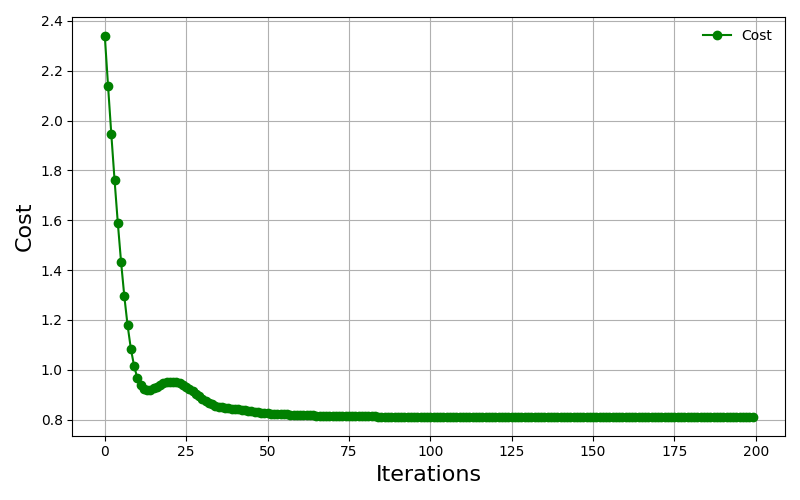
\includegraphics[width=80mm]{task3-cost.png}
    \caption{Cost history}
    \label{fig:enter-label}
\end{figure}

\textbf{\textcolor{red}{After fixing a mistake in the definition of softmax cost function, below is the correction: }}
\begin{figure}[H]
    \centering
    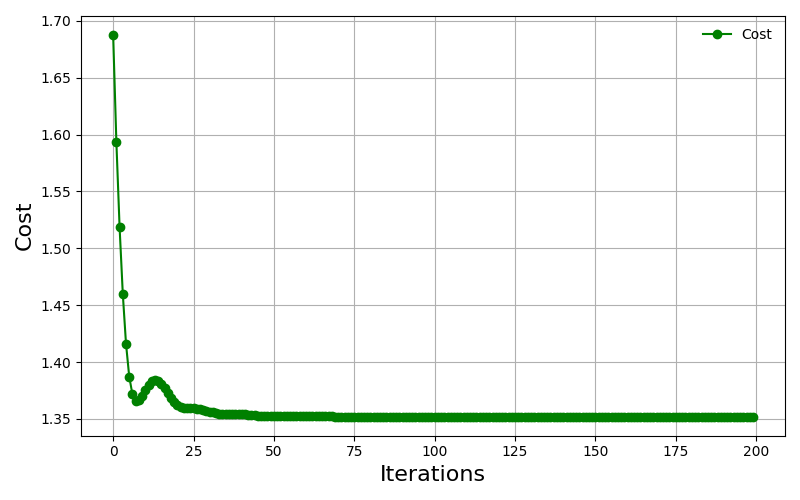
\includegraphics[width=80mm]{task3-cost-corrected.png}
    \caption{Cost history}
    \label{fig:enter-label}
\end{figure}

\textbf{2.} The final cost and accuracy of your solution to the 4-class classification task
\begin{table}[H]
    \centering
    \begin{tabular}{|c|c|c|}
    \hline
        Final cost & 0.8115 & \textbf{\textcolor{red}{1.35197; after correction}}\\
        Misclassifications &  11 & \textbf{\textcolor{red}{8; after correction}}\\
        Overall accuracy &  72.5\% & \textbf{\textcolor{red}{80\%; after correction}}  \\
    \hline
    \end{tabular}
    \caption{Model performance}
    \label{tab:my_label}
\end{table}

\textbf{3.} A figure showing the original data and regions of your model solution
\begin{figure}[H]
    \centering
    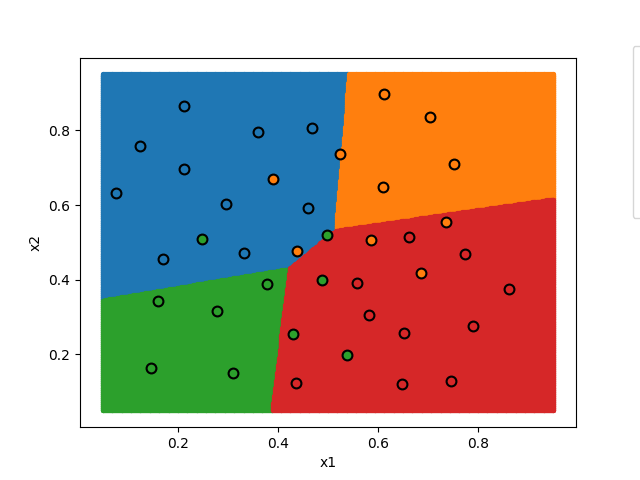
\includegraphics[width=120mm]{classifier_label_regions.png}
    \caption{Final Model}
    \label{fig:enter-label}
\end{figure}


\textbf{\textcolor{red}{After fixing a mistake in the definition of softmax cost function, below is the correction of the final classification: (only 8 misclassifications)}}
\begin{figure}[H]
    \centering
    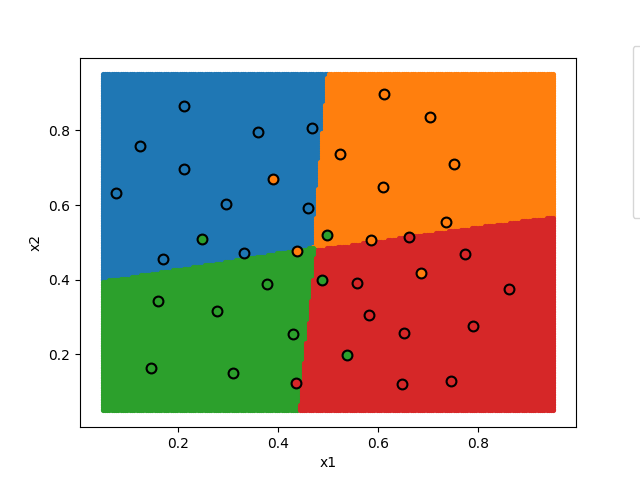
\includegraphics[width=120mm]{classifier_label_regions-corrected.png}
    \caption{Final Model}
    \label{fig:enter-label}
\end{figure}










